\chapter{\acl{sota}}
\label{chapter:sota}

\section{Datasets}
\label{section:sota:datasets}

Training an autonomous vehicle to be capable of driving itself is a complex challenge with multiple parts and problems to solve: recognizing other road users (people, vehicles, cyclists); understanding traffic signs; track and estimate the movement of the road users; plan the path; accurate modelling of the environment; among many others. To both train neural networks and other genetic algorithms, but also to test systems and other software, huge amounts of data are required.

To accelerate this progress, a collaborative effort is being made to release free datasets online for public usage under permissive licenses. These datasets vary in their objective, sensory data available, conditions which data has been acquired, driving conditions and format on which they are provided, among other aspects. 

Despite this work not intending to study autonomous driving, the algorithms developed for calibration, sensor fusion and computing the correspondence between objects of interest in image and point cloud are not meant to be particularly applied on datasets with interference. Therefore, using public available datasets not only allows the development of those algorithms before experimental data can be gathered, but also widen the applicability of such work, without losing their applicability to the particular situation of \ac{lidar} interference.

During the months when this research work was carried, several new datasets were made available online, such as nuScenes~\cite{nuScenes2019} and Waymo~\cite{Waymo}. Since no new contribute to this research was expected from their usage, no further research on them was carried. 

Several datasets were considered and tested. On the next sections, a brief summary is given about the ones that have sensory data from camera and \ac{lidar}. Those were the candidates to be used on this work.

\subsection{Ford Campus \acl{lidar} dataset}
Gathered in 2009, in Michigan, the Ford Campus \ac{lidar} dataset contains camera, \ac{lidar}, \ac{imu} and \ac{gps} data. The dataset consists of two test scenarios, one inside the Ford Research campus and the other on downtown Dearborn. A small subset of the former test scenario is also provided.

The data is provided in raw format, accompanied by log files with timestamps, \ac{gps} and \ac{lcm}\footnote{For more information on \acf{lcm} protocol for estimating delays between sensory data registration on master-slave systems, see~\cite{VelodyneHDL64}.} logs with all raw data. The images from an omnidirectional camera, a Point Grey Ladybug3, are stored on \ac{ppm}; \ac{lidar} data from a Velodyne HDL-64E on \ac{pcap} format, from the \ac{tcp} connection socket; two Riegl LMS-Q120 \acp{lidar} also provide more information on the scan.

Rectified and synced data is stored under \ac{matlab} \textit{.mat} files. Along with the raw data and synced and rectified \textit{.mat} files, source code is also provided for parsing the raw data, visualizing the \ac{lcm} logs and pre-processed data on \ac{matlab}. A C and \ac{opengl} software that can render textured point clouds is also available.

The modified Ford F-250 pickup truck, which can be seen on figure~\ref{fig:sota:ford_sensors}, uses 3 sensors for navigation~\cite{Pandey2011}: one 3D \ac{lidar}, Velodyne HDL-64E \ac{lidar}~\cite{VelodyneHDL64}; one camera: Point Grey Ladybug3 omnidirectional camera; and two 2D \acp{lidar}: Riegl LMS-Q120 lidar. For more details about the sensors, their relative positioning, data formats and files see~\cite{Pandey2011}.

\begin{figure}
	\centering
	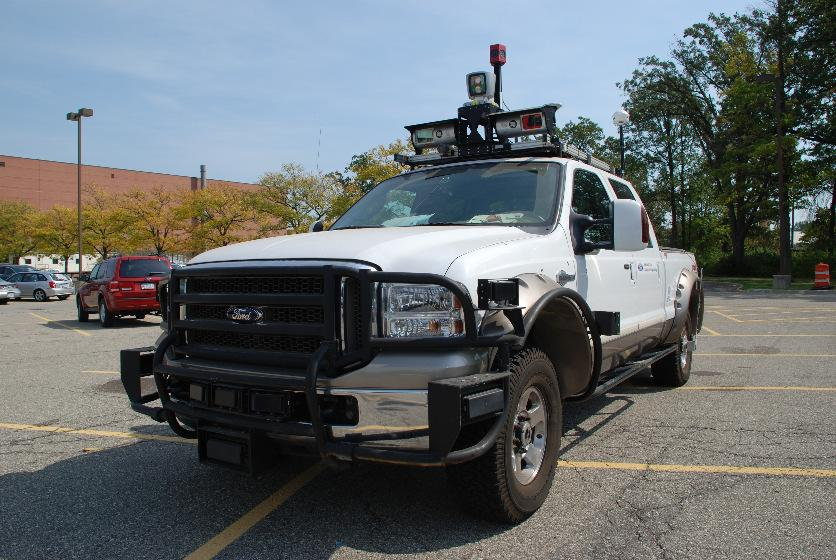
\includegraphics[width=0.5\textwidth]{img/sensor_fusion/ford_sensors.jpg}
	\caption{Ford 250 pickup equipped with the sensors described in the previous paragraphs. On the top, the Ladybug omnidirectional camera, on the back the \ac{imu} and \ac{gps} unit.}
	\label{fig:sota:ford_sensors}
\end{figure}


\subsection{\acl{kitti} Dataset}
A well known dataset for researchers of computer vision, autonomous driving and \ac{ml}, \ac{kitti} was recorded in 2011 and released to the public in 2013. This dataset contains various driving scenarios: suburban, highways, residential and campus areas; with trucks, cars, cyclists and persons. Alongside with data for testing, calibration measures are provided for all sensors.

The test car, a Volkswagen Passat is equipped with two stereo pairs, one with color and one with gray cameras, a \ac{lidar}, an \ac{imu} and a\ac{gps} sensor. Data from all four cameras is stored on \ac{png} format, \ac{lidar} measurements stored as a binary float matrix, \ac{gps} and {imu} ares saved textually. Additionally, the raw data logs containing the timestamps and the transformations between the sensors are also provided. Labeled data is also available for some test scenarios on \ac{xml} files.

Along with the data and calibration parameters, several tools written in C++ or \ac{matlab} are also provided. The dataset offers two types of data categories: (1) unsynced and unrectified data or (2) synced and rectified data. 

The sensory apparatus contains 2 PointGray Flea2 greyscale and color cameras, a Velodyne HDL-64E \ac{lidar}~\cite{VelodyneHDL64}, among others less relevant sensors~\cite{Geiger2013a}.

\begin{figure}
	\centering
	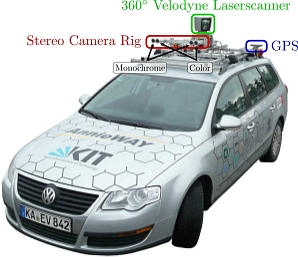
\includegraphics[width=0.5\textwidth]{img/sensor_fusion/passat_sensors.jpg}
	\caption{Volkswagen Passat equipped with the sensors described in the previous paragraphs, for the \ac{kitti} dataset. On the top, the Velodyne \ac{lidar} and below the 2 stereo pairs (color and grey). On the back, the \ac{imu} and {gps} systems are present.}
	\label{fig:sota:kitti_sensors}
\end{figure}


\subsection{Udacity Self-Driving Car Nanodegree Dataset}
the data from Udacity online course on self-driving car is also publicly available. This dataset dates to 2016 and was gathered to develop a level 4 autonomy vehicle, containing much more data diversity than the previous two. The data available contains images from 3 color cameras,  \ac{lidar}, \ac{imu} and \ac{gps}, among other sensory data, such as speed, braking, etc.

This information is not available in raw format, only structured in \ac{ros} \textit{.bag} files. Some tools for visualizing and interacting with their data are provided for \ac{ros}~\cite{udacity}. 

Not much information about the sensors and their positioning positioning is publicly available, and the dataset does not contain information for calibration.

\subsection{Summary}
Table~\ref{tab:sota:datasets_comparison} summarizes all the relevant data from the datasets~\cite{udacity, Pandey2011, Geiger2013a}. While there are few differences between the relevant types of data gathered, major differences can be observed on the format in which they are provided. 

The diversity of scenarios and size of the dataset is also an aspect to consider. On this matter, \ac{kitti} and Udacity's are superior to Ford dataset, with \ac{kitti} providing the largest dataset in quantity, with already rectified and synced data. 

While Udacity dataset is the newest and provides direct out-off-the-shelf integration with \ac{ros}, that type of integration can also be achieved for \ac{kitti} by using other tools, such as \textit{kitti2bag}~\cite{TomasKrejci}. 
	
\begin{table}[H]
	 \rowcolors{4}{gray!10}{white}
	 \renewcommand{\arraystretch}{1.2}
	 \centering
	\begin{tabular}{llccc}
																& & \multicolumn{3}{c}{Datasets} \\ \cline{3-5}
																& & Ford Campus  & \acs{kitti} & Udacity \\ \midrule
																%
																& \ac{lidar}	   & \checkmark  & \checkmark & \checkmark \\ 
																& Color Camera	 & \checkmark  & \checkmark & \checkmark  \\
																& Grey Cameras   &             & \checkmark &  \\
																& Stereo Camera  &             & \checkmark & \checkmark  \\
																& Omnidirectional Camera &  \checkmark  &  &  \\
																& \acs{imu}      & \checkmark  & \checkmark & \checkmark  \\
																& \acs{gps}      & \checkmark  & \checkmark & \checkmark  \\
		\rowcolor{white}\multirow{-8}{*}{Sensors and Data} & Driving data\footnotemark & & & \checkmark \\ \hline
		\multirow{5}{*}{Data Formats and Tools} & Raw data available & \checkmark & \checkmark &  \\
																			 & Data parsing tools & \checkmark & \checkmark & \checkmark  \\
																			 & Rectified data & \checkmark & \checkmark & \checkmark \\
																			 & Synced data & \checkmark & \checkmark &  \checkmark  \\ 
																			 & Calibration parameters & \checkmark  & \checkmark  & \checkmark  \\\hline 
		\multicolumn{2}{l}{Raw data for sensors calibration} & \checkmark & \checkmark & \\
		\multicolumn{2}{l}{Direct \ac{ros} data compatibility} &  & \checkmark & \checkmark \\
		\multicolumn{2}{l}{Date of acquisition} & 2009  & 2011 & 2016 \\
		\bottomrule
	\end{tabular}
\caption{Comparison between the datasets more appropriated to this thesis objectives}
\label{tab:sota:datasets_comparison}
\end{table}
\footnotetext{Other driving data includes, but it is not limited to: vehicle speed, joints states, twist, brakes, suspension, fuel level, \ac{can} bus data, steering, tire pressure, among many others.}

Comparing the 3 datasets, not only using table~\ref{tab:sota:datasets_comparison} but also the previous sections, Udacity and \ac{kitti} are more suited to the purposes of this work. They provide a larger dataset than Ford, have \ac{ros} compatibility and the tools provided are open-source and not developed to be used on proprietary software.

Since Udacity dataset integrates more easily with \ac{ros} than \ac{kitti}, providing also some tools for \ac{ros} preliminary tests, learning and earlier development stages will occur with this dataset. Later, due to the lack of calibration parameters and raw data for sensors calibration\footnote{Note that, despite Udacity dataset not providing data to ease the calibration of its sensors, such as camera intrinsic calibration or the extrinsic calibration between \ac{lidar} and camera, such calibration parameters can be obtained from this data. Those parameters are not accurate as those obtained using a proper calibration setup and are out the scope of this research (being another research topic on itself) and therefore no effort will be dedicated to this topic.}, this research will use the \ac{kitti} dataset.


%%%%%%%%%%%%%%%%%%%%%%%%%%%%%%%%%%%%%%%%%% CAMERA %%%%%%%%%%%%%%%%%%%%%%%%%%%%%%%%%%%%%%%%%%

\section{Camera as a sensor on \acl{cv} applications}
Vision is the human sense most relevant to how we perceive the world and how we navigate it~\cite{Ekstrom2015, Beck1983}. Replicating this ability on machines, through the usage of cameras, is a widely researched topic on computer vision and instrumentation~\cite{Beck1983}. The most common cameras, as our eyes, take advantage of the pinhole effect: a small hole (or pin), that is used to spatially filter the non-focused light beams through an aperture or lens~\cite{Beck1983, camera_models, Sturm2010}, producing a mirrored, but focused image.

On the following sub sections, basic notions of the current status of camera models and camera calibration are given. Since this research is focused strictly the application a camera as sensor on computer vision, the overview provided abstains from describing extensive research on camera technologies and camera models for the field of computer vision. From a purely working principle and technologies, several camera types can be named, such as catadioptric, plenoptic, biprism, among others~\cite{Sturm2010}. Considering consumer market, denominations such as Compact Cameras, \ac{dslr} cameras, Mirrorless (or \ac{evil} cameras) can also be used~\cite{comercial_cameras}. For further research, the reader might be interested on~\cite{comercial_cameras, Sturm2010, camera_models, Merklinger1993, Photopillers}.


\subsection{Camera Geometry}
A world point in a 3-dimensional Euclidean space can be represented by a vector with 3 real coordinates: $(X, Y, Z)$ and an image pixel of a digital image is typically represented as an element of a 2D matrix with integer coordinates $(u, v)$~\cite{mvg_book}. From a mathematical standpoint, a camera can be considered as a mapping tool between the world objects in three dimensions into a 2D image plan, such as depicted by equation~\ref{eq:camera_transform}, which as different resolutions depending on the mathematical model used to describe the camera~\cite{mvg_book, Sturm2010}.

\begin{equation}
	\label{eq:camera_transform}
	(X, Y, Z) \xrightarrow[]{\text{transformation}} (u, v)
\end{equation}

When describing camera models, several considerations should be made~\cite{Sturm2010}:
\begin{itemize}
	\item \textbf{Central Camera Models vs Non-Central Camera Models}: quantifies the number of optical centers on a camera. A central camera as only one optical center through which all light rays pass through to reach the film and a non-central has two or more optical centers;
	\item \textbf{Global vs Local models:} indicates if the parameters of the model are the same for all the image/\ac{fov} of the camera or different regions of the image have different parameters, respectively;
\end{itemize}

For the application currently envisioned, global central camera models are considered. For a more detailed explanation of the topics above or an extensive overview of non-classical camera models, different types of projections and other aspects of modelling cameras, see~\cite{Sturm2010, camera_models}.

\subsubsection{Pinhole Camera Model}
Based on the pinhole effect, represented on figure~\ref{fig:pinhole_effect}, the pinhole camera model is the most common camera model~\cite{camera_models}. The pinhole effect consist on using a small hole (or aperture) to spatially filter the light rays by angle of incidence, reducing the amount of light rays overlapping when coming from different incident angles through the pinhole, which would create noise and ``blur'' the image. 

\begin{figure}[H]
	\centering
	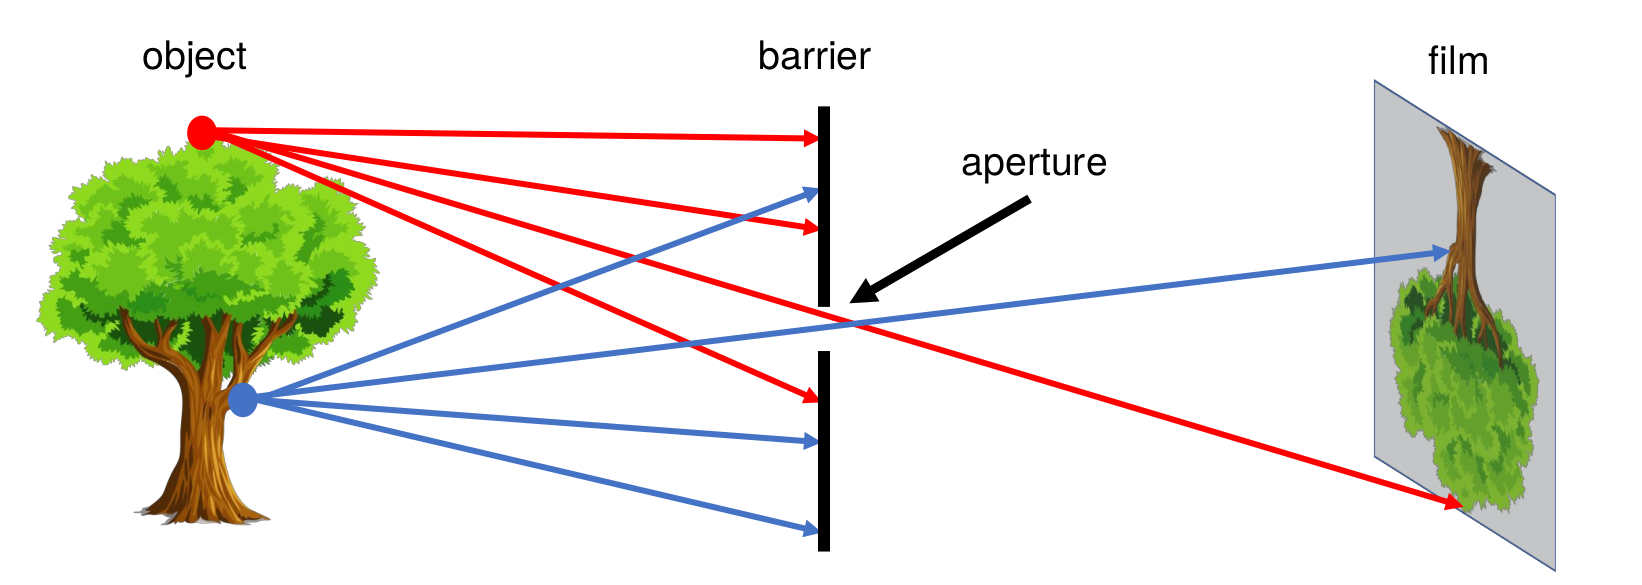
\includegraphics[width=0.6\textwidth]{img/camera/pnhole_effect.png}
	\caption{Pinhole effect on a small aperture. Source:~\cite{camera_models}}
	\label{fig:pinhole_effect}
\end{figure}

The pinhole camera model describes the perspective transformation on equation~\ref{eq:camera_transform} as a central projection where all light rays meet at the camera center, $\mathcal{F}_c$. A diagram of the pinhole camera is shown on figure~\ref{fig:pinhole_camera_model}. 

On this model, the z-axis is collinear with the optical axis\footnote{Also called principal axis. The two terms can be changed with no loss of context.}, aligned with the direction the camera is facing. The image plane is at $z = f$, where $f$ is the focal length, being intersected by the optical axis on the principal point, with coordinates $(c_x, c_y)$ on the image plane axis. Note that the principal point is not the origin of the referential on the image plane, but instead the middle point, being the origin located in the top left corner, with a downward y-axis.

\begin{figure}[H]
	\centering
	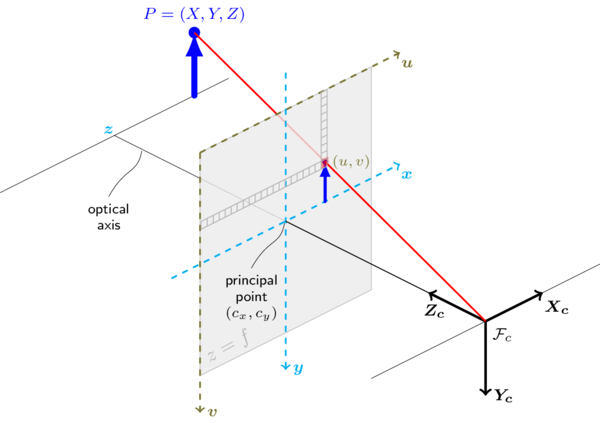
\includegraphics[width=0.6\textwidth]{img/camera/pinhole_camera_model.png}
	\caption{Pinhole camera model. Source: \acl{opencv}\cite{opencv_doc}}
	\label{fig:pinhole_camera_model}
\end{figure}

Due to the nature of the pinhole camera model, is more convenient to use a Projective Space instead of the more common Euclidean Space\cite{mvg_book, camera_models, Sturm2010}. On a Projective Space, as in a central camera model, all of its points are oriented through a single point~\cite{mvg_book}. Therefore, by using a projective space instead of a Euclidean for addressing the transformations of a pinhole camera model, mathematics become more intuitive and relatable to the actual geometry of the model. Projective spaces use homogeneous coordinates and has non-Euclidean geometry, but that allow for changes between the two\cite{mvg_book, camera_models}.

\subsubsection{Projective Geometry}
A tridimensional Euclidean Space can be represented on a Projective space using 3+1 coefficients. Therefore, the previous tridimensional vector can be rewritten in homogeneous coordinates as $(wX, wY, wZ, w)$ \cite{mvg_book}. If $w \neq 0$, we can transform from the Projective to Euclidean Space, obtaining the world representation of such points, by dividing the homogeneous point by $w$. For the cases in which $w =  0$, we have purely projective points at infinity, that only exist in Projective Space~\cite{mvg_book}. 

The relation depicted in equation~\ref{eq:camera_transform} can expressed in projective geometry as:

\begin{equation}
	\begin{bmatrix}
		u \\ v \\ 1
	\end{bmatrix}
= P \times 
\begin{bmatrix}
		X \\ Y \\ Z \\ 1
	\end{bmatrix}, \qquad \text{if } w = 1
\end{equation}

$P$ represents the projection matrix that performs the transform from world points to image pixels. The projection matrix in a pinhole camera model is the result of multiplication of two matrices: the camera matrix (or matrix of the camera intrinsic parameters), $K$; and a joint rotation and translation matrix, $[R|t]$ - where $R$ is the rotation matrix and $t$ the translation vector. The combination of these matrices is given on equation~\ref{eq:projective_matrix} and the full camera transform is expanded on equation~\ref{eq:camera_transform_full}, through the replacement of equation~\ref{eq:projective_matrix} in~\ref{eq:camera_transform}.

\begin{equation}
	\label{eq:projective_matrix}
	P = K[R|t]
\end{equation}

\begin{equation}
	\label{eq:camera_transform_full}
	\begin{bmatrix}
		u \\
		v \\
		1
	\end{bmatrix}
	= 
	\overbrace{
		\underbrace{
			\begin{bmatrix}
				f_x & 0 & c_x \\
				0 & f_y & c_y \\
				0 & 0 & 1 
			\end{bmatrix}
		}_\text{\large\textbf{K}}
		\underbrace{
			\left[
				\begin{array}{ccc|c}
					r_{xx} & r_{yx} & r_{zx} & t_x \\
					r_{xy} & r_{yy} & r_{zy} & t_y \\
					r_{xz} & r_{yz} & r_{zz} & t_z 
				\end{array}
		\right]
		}_\text{\large\textbf{[R|t]}}
	}^\text{\large\textbf{P}}
	\begin{bmatrix}
		X \\
		Y \\
		Z \\
		1
	\end{bmatrix}
\end{equation}

The intrinsic parameter matrix is used to represent the calibration parameters of the camera, namely, the focal lengths of each axis, $f_x$ and $f_y$, and the principal point offset to the axis origin, $c_x$ and $c_y$, for the x and y-axis, respectively. The joint rotational-translation matrix, $[R|t]$, is also known as the extrinsic camera parameters, translates the coordinates of a point to the Cartesian coordinate system fixed to the camera.


\subsubsection{Cameras, Lenses and Distortion}
Using a simple pinhole for filtering light rays that would cause noise on the image severely reduce the amount of reaching the camera receptor. Therefore, a lens is used to steer the light and provide the same effects as the hole~\cite{Sturm2010}. The pinhole effect with a lens can be seen on figure~\ref{fig:pinhole_with_lense}.

\begin{figure}[H]
	\centering
	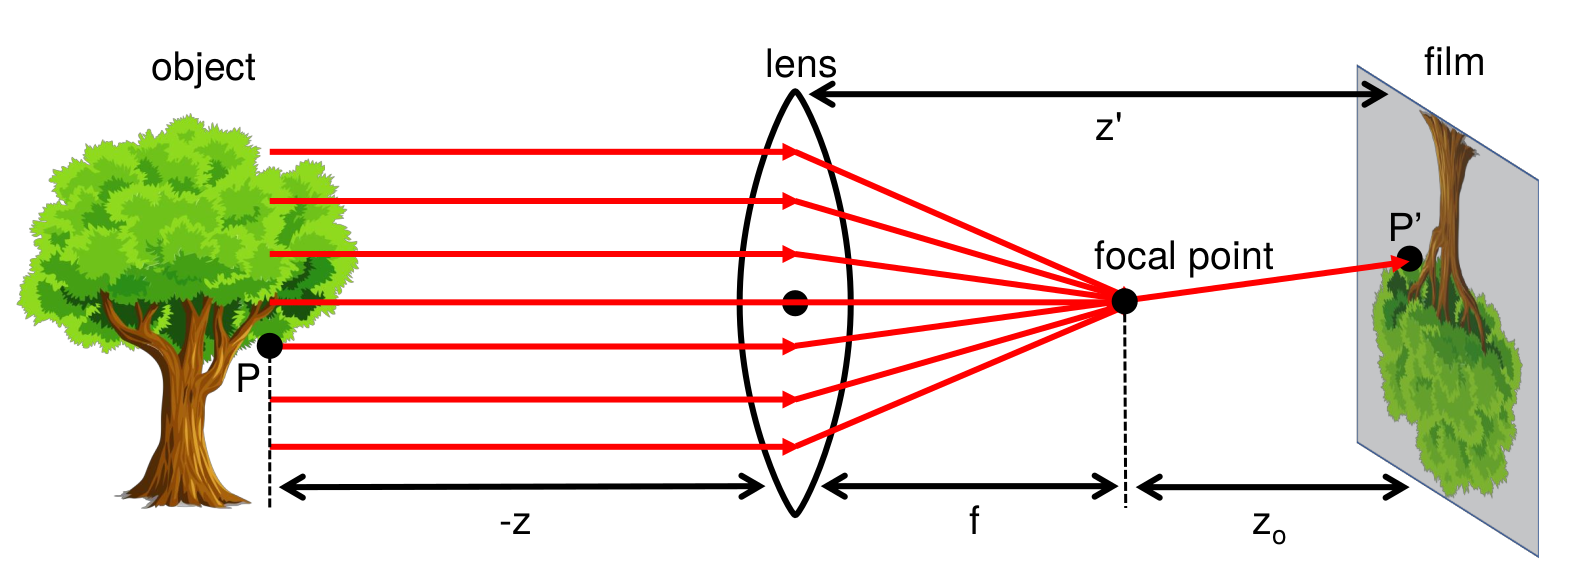
\includegraphics[width=0.6\textwidth]{img/camera/pinhole_with_lense.png}
	\caption{Pinhole effect on a lens. Source:~\cite{camera_models}}
	\label{fig:pinhole_with_lense}
\end{figure}

Since lenses introduce non-linear distortion, the pinhole camera model needs to be extended to included radial and tangential distortion parameters~\cite{Bouguet2010, manuapphotogrammetry, Heikkila1997}. Such parameters indicate how the non-linear distortion of the camera lenses affects the image projection on the camera plane~\cite{camera_models, Sturm2010} and how can this be corrected~\cite{Heikkila1997, Bouguet2010, opencv_doc}. The equations behind that expression are behind the scope of this introduction and therefore will not be detailed here, but the effect of lens aberration can be seen on figure~\ref{fig:lense_distortion_types}, extracted from Hata and Savarese course notes~\cite{camera_models}.

\begin{figure}[h]
	\centering
	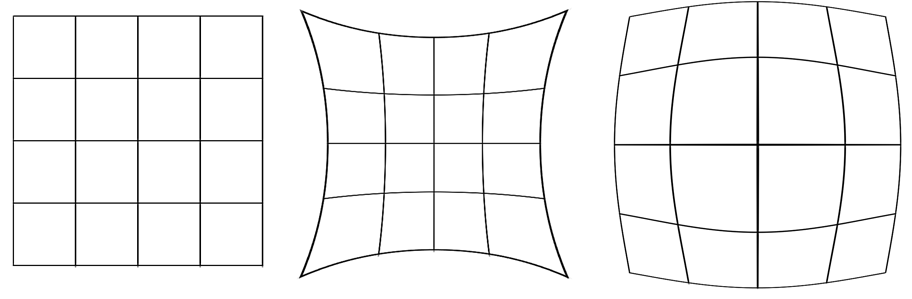
\includegraphics[width=0.5\textwidth]{img/camera/distortion.png}
	\caption{Examples of barrel and pincushion distortion on an image. Source: \cite{camera_models}}
	\label{fig:lense_distortion_types}
\end{figure}

For more information on the pinhole camera model and lens distortion, see Hartley and Zisserman Multi View Geometry in Computer Vision~\cite{mvg_book}, Hata and Savarese course notes\cite{camera_models} or \acf{opencv} official documentation\cite{opencv_doc}. 

\subsection{Camera Intrinsic Calibration}
\label{subsec:sota:camera-intrinisc-calibration}
Calibrating a camera is the process on which the parameters of the model that describes its behavior are determined. For the extended pinhole camera model, this means determining the parameters of its intrinsic matrix, $K$, but also the distortion coefficients of the lens used~\cite{mvg_book, camera_models, Bouguet2010, Heikkila1997}. These parameters are called the intrinsic parameters and are independent of the scenario being viewed, if the focal length is kept constant. On the other hand, extrinsic camera parameters are different for every situation and therefore scenario dependent~\cite{opencv_doc, Bouguet2010, Heikkila1997}.

Zhang proposed in 2000 a method for calibrating a camera that unlike previous others\citeneeded, does not require a special setup, expensive experimental apparatus or complicated calibration patterns: it uses a planar object with a known pattern, which can be freely moved in front of the camera~\cite{Zhang2000}. Only two images are necessary for camera calibration, as long the pattern movement between them is not a pure translation. The estimation of the camera intrinsic parameters and distortion caused by the lenses can be determined by solving the equation~\ref{eq:camera_transform_full}, once the $2D \leftrightarrow 3D$ correspondences have been established.

The correspondences between the 2D and 3D representations of the pattern can be made by finding the corners or circles on planar patterns~\cite{opencv, mvg_book}. Chessboards are the most common patterns used today~\cite{opencv}, allowing corner detection for each cell. Since the dimensions of the cell and their arrangement is known previously, it is possible to compute the orientation of the chessboard~\cite{Zhang2000, opencv_doc, mvg_book}. On that conditions, revisiting equation~\ref{eq:camera_transform_full}, only the $K$ matrix is left to be determined. An example is a chessboard calibration pattern with is interest point for calibration is shown on figure~\ref{fig:opencv_calib_pattern}.

\begin{figure}
	\centering
	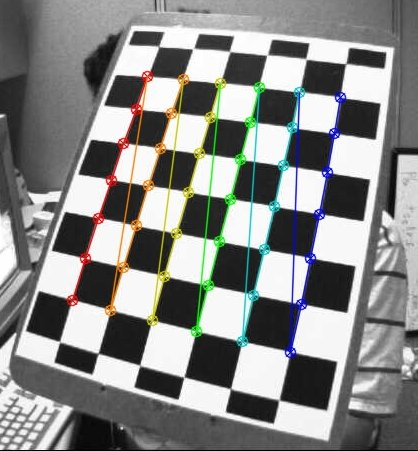
\includegraphics[width=0.4\textwidth, keepaspectratio]{img/camera/calib_pattern.jpg}
	\caption{Chessboard calibration pattern with corners detection results show on image. Corner order is also given on the corner color. Source:~\cite{OpenCV_camera_calib}.}
	\label{fig:opencv_calib_pattern}
\end{figure}

This estimation can then be refined using a maximum-likelihood estimation to minimize the error using a non-linear method, such as Levenberg-Marquardt optimization~\cite{Levenberg1943}. Other optimizations are possible, such as Powell’dog-leg non-linear least squares technique~\cite{Lourakis2005}. Further reading can be conducted on~\cite{mvg_book, Sturm2010, camera_models, Hata, Xu1996a}.

Zhang's algorithm differs from other methods at the time that attempted to calibrate a camera by rotating it on a static environment~\citeneeded. Other alternative algorithms include Tsai's algorithm \cite{Roger1987, mvg_book}, a 2-stage technique for camera calibration first presented in 1987, that does not determine the camera center. A \ac{dlt} algorithm can also be used to determine the camera calibration parameters (see~\cite{mvg_book}).

Bouguet in 2010 provides a Camera Calibration toolbox for \ac{matlab}~\cite{Bouguet2010}, which serves as the basis for many camera calibration toolboxes, such as \ac{opencv}, which is based on the works of Bouguet and Zhang~\cite{opencv}.


\subsection{Camera as a sensor for computer vision}
On the field of computer vision, several tools and libraries are available, capable of performing low image operations, image detection, filtering, among others. 

\begin{itemize}
	\item \textbf{BoofCV~\cite{boofcv}:} written in java, this library is oriented to real-time image operations, such as low-level image processing, camera calibration and feature/object  detection, tracking and recognition;
	\item \textbf{Dlib~\cite{dlib}:} modern C++ toolkit containing \acl{ml} algorithms and tools, some on the field of computer vision;
	\item \textbf{\ac{matlab} Computer Vision Toolbox\texttrademark~\cite{matlabcvtoolbox}:} toolbox for computer vision algorithms, 3D vision, and video processing systems. Can be performed object detection and tracking. Detects, extracts and matches features;
	\item \textbf{\acf{opencv}~\cite{opencv}:} open source library for C++, Python and C that implements \acl{sota} algorithms on computer vision;
	\item \textbf{Vlfeat~\cite{vlfeat}:} open source library for C that implements many \acl{sota} algorithms on computer vision;
	\item \textbf{SimpleCV~\cite{simplecv}:} Open source framework, written in python, that can be used to implement computer vision software using other libraries;
\end{itemize}

Since a goal of this research is to use Open-Source tools as far as possible (instead of using closed source tools or code that is harder to integrate with other libraries), \ac{matlab} \acl{cv} Toolbox\texttrademark~does not suit. The code of this research is mainly develop in C++ (see chapter \citeneeded), so Python and Java libraries will not be considered, resulting only in \ac{opencv} and Dlib (Vlfeat uses plain C, so also not ideal). 

\ac{opencv} has a great community and is considered by many researchers and industry leaders as the \textit{de facto standard} library when refereeing to computer vision. Dlib is a robust library, but no significant differences can be when comparing with \ac{opencv}. Therefore, the final choice for a computer vision library is \ac{opencv}, due to the already implemented compatibility with \ac{ros}.



%%%%%%%%%%%%%%%%%%%%%%%%%%%%%%%%%%%%%%%%%%% LIDAR %%%%%%%%%%%%%%%%%%%%%%%%%%%%%%%%%%%%%%%%%%

\section{Automotive \ac{lidar}}
\ac{lidar} sensors map their surroundings thanks to their capability of precisely measuring depth. Already used in topography, spectrography and air pollution studies, \ac{lidar} found its importance on the automotive industry as one of the sensors of autonomous cars and \ac{adas}\cite{Sullivan2016}. 

These maps produced by the \ac{lidar}, commonly represented as point clouds or mesh clouds models, (see figure~\ref{fig:bunny}), are one of the preferred method for \ac{slam} algorithms, which allow a vehicle without previous knowledge of its surroundings to autonomously navigate them, a crucial task for \ac{adas} on self-driving vehicles.

\begin{figure}[H]
	\centering
	\begin{subfigure}[c]{0.45\textwidth}
	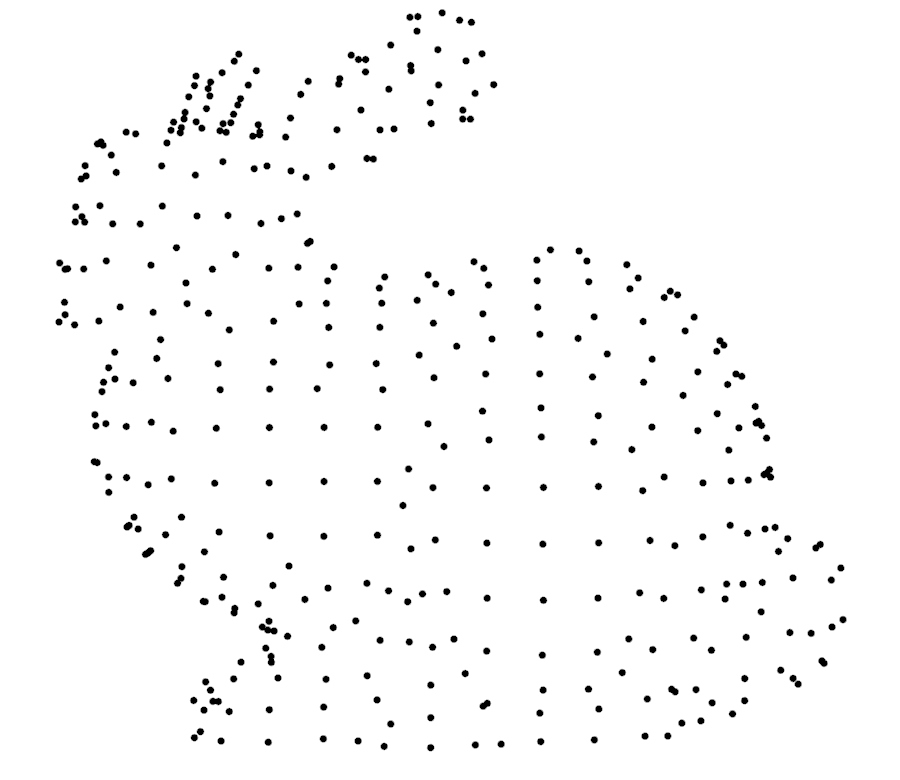
\includegraphics[width=\textwidth]{img/lidar/bunny_point.png}
		\caption{Point Cloud representation}
		\label{fig:bunnyPointCloud}
	\end{subfigure}
	\quad
	\begin{subfigure}[c]{0.4\textwidth}
		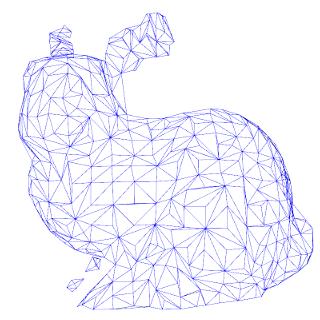
\includegraphics[width=\textwidth]{img/lidar/bunny_mesh.png}
		\caption{Mesh Cloud representation}
		\label{fig:bunnyMeshCloud}
	\end{subfigure}
	\caption{Stanford bunny~\cite{bunny} point cloud (\subref{fig:bunnyPointCloud}) and mesh cloud (\subref{fig:bunnyMeshCloud})}
	\label{fig:bunny}
\end{figure}


Typically, four major technologies are used on the construction of a \ac{lidar}~\cite{Hecht2018, Sullg}:

\begin{enumerate}
	\item \textbf{\ac{tof}:} the most common type, acquires depth information by measuring the time elapsed between the emission and reception of a \ac{laser} pulse reflected from a surrounding target \cite{Sullivan2016};
	\item \textbf{Flash~\cite{Ouster, Gelbart2002,Stettner2010, Simpson2019}:} organized in a matrix structure, similar to a camera \ac{ccd}, every element of the matrix contains a photodetector. A ``flash'' simultaneous illuminates all the \ac{fov}, and the reflected light intensity and time of arrival is measured to provide depth calculations; 
	\item \textbf{Phased Arrays~\cite{Quanergy2018, Yu2016}:} using a microscopic array of antennas, similar to a \ac{radar}, the phase of each antenna is controlled to allow the \ac{lidar} to sweep and/or focus on a specific area, using beamforming theory;
	\item \textbf{\ac{mems}:} operate by controlling the angle at which a rotating microscopic mirror is aligned with the \ac{laser}. By varying the angle a single line can be scanned and using multiple \acp{laser} with the same mirror allows vertical scan.
\end{enumerate}


\subsection{\acl{tof} vs Solid State \acp{lidar}}
Despite the existence of several technologies that can be used for \ac{lidar} construction, two major types of \ac{lidar} can be distinguished: \ac{tof} or Solid State~\cite{Hecht2018}. The former as no moving parts while the latter working principle is the rotational device.

To construct a \ac{tof} \ac{lidar}, a single pair of \ac{laser} and photodetector is assembled on a fast rotational device (typically 5 to 20 Hz), allowing that pair to measure a single line while rotating, creating a 2D \ac{lidar}. If multiple pairs are assembled together, with different polar angles, on a rotational device, the \ac{lidar} is said to be a 3D \ac{lidar}, since a total revolution can produce a three-dimensional map of its surroundings~\cite{Sullivan2016}.

Solid State \ac{lidar} has no moving parts, and can either use flash or phased arrays on its construction, depending on a flash of light to illuminate the scene or performs beam steering to scan the same scene. They are theoretically more reliable, durable cheaper and consume less power. However, this technology is not yet mature, which makes the current models impractical for automotive~\cite{Fersch2017a}. 

While \ac{tof} \acp{lidar} consumes more power, they can also achieve ranges until 100 meters \cite{vlp16, Sullivan2016} or even 200 meters\cite{VelodyneHDL64, Sullivan2016}, higher than solid state \ac{lidar}, which is still on laboratory tests and development, with the first prototypes reaching 2 meters~\cite{Hecht2018}. That is due to the attenuation of the flash intensity, due to its power being inversely proportional with the distance squared or losses in the phased array. Considering the current \ac{sota} on \ac{tof} \ac{lidar} has less error (a few centimeters) than the \ac{sota} of Solid State \ac{lidar}~\cite{Hecht2018, Fersch2017a}.

However, Solid State \ac{lidar} have more point density than a \ac{tof} counterpart and measure the depth image of a scene on the same frame, theoretically allowing for more accurate data and faster refresh rates\cite{Sullivan2016, Hecht2018, Fersch2017a}



%Combining the reliability of the depth measurement with the assemblage of multiple pairs of \ac{laser} and photodetectors on a fast rotational device (typically 5 to 20 Hz) creates one of the most appealing and reliable sensors for self-driving vehicles and \ac{adas}.

%Despite the relevance of the topic for the massification of self-driving vehicles and the hazardous impact on \ac{adas} reliability, the research topic presented in this paper has received reduced attention by the research community. 
%A major \ac{lidar} manufacture also addresses the problem of mutual interference of the \ac{lidar} sensors on the same vehicle, by allowing their synchronization and \ac{laser} firing in different instants \cite{vlp16}.


\section{Camera and \ac{lidar} Extrinsic Calibration}
\label{sec:sota:extrinsic_calibration}

On a multiple sensor setup, coordinated frames from one sensor must be able to be referred on another sensor reference frame. Transforming data from one frame to another requires performing extrinsic calibration between them, by determining the rigid body transform~\citeneeded that can convert the data from one reference plan to the other without lost of meaning. 

Therefore, the sole purpose of extrinsic calibration is to determine the coefficients of this transform, that can be described as a rotation and a translation, similarly to the joint rotation-translation matrix $[R|t]$ used for camera intrinsic calibration (equation~\ref{eq:camera_calibration_full}). However, on this case, instead of this matrix representing the rotation of the object to the camera or the camera movement in the world, it represents the rotation and translation operations that need to be applied to the coordinate system of one sensor (and its data) to align the data with the coordinate system of another sensor. The precision of this transformation takes particular interest when data fusion (or sensor fusion) is trying to be achieved, i.e., merging from this data sources o reduce errors and improve the significance of data each sensor is capable of giving~\citeneeded. 

Several algorithms have been suggested for performing extrinsic calibration on data. They range from the necessity of well controlled environments to require no human intervention, using or not a calibration pattern. 


\subsection{Calibration using Patterns}
Typical extrinsic calibration between \ac{lidar} and camera with intersecting \ac{fov} use calibration patterns: Unnikrishnan first proposed a \ac{lidar}-Camera extrinsic calibration using a toolbox developed to manually selected correspondences between a calibration pattern on image and point cloud~\cite{Unnikrishnan2005}. A \ac{matlab} toolbox to ease the process has also developed in 2005 from Unnikrishnan \etal. Fremont \etal uses a planar calibration target with a hole surrounded by a solid color, matching the depth discontinuities from the \ac{lidar} with the color discontinuities from the camera \cite{Fremont2013} and Velas uses a planar pattern with geometric objects carved on its surface~\cite{MartinVelas2013}. Liao \etal proposes a method that only requires the usage of a planar polygon of known shape~\cite{Liao2019} and Park \etal tests and presents results of this calibration method applied to multiple polygons, specially with triangular shape~\cite{Park2014}. Mirzaei \etal uses a planar pattern with fiducial marker~\cite{Mirzaei2012}. 

Regarding calibration with three-dimensional calibration targets, Pusztai uses a box with different colors on each face~\cite{Pusztai2018}; Pereira a ball (for performing multiple sensor calibration, instead of only 3D \ac{lidar} and monocular camera)~\cite{Pereira}; Gong a trihedral object, determining the extrinsic calibration parameters using a nonlinear least squares algorithm~\cite{Gong2013}.

While the previous methods where focused on calibrating monocular cameras with tridimensional \ac{lidar}, alternative methods exist for stereo systems, taking advantage of the disparity map obtained with a stereo camera. Automatic methods are proposed by Geiger \etal and Guindel \etal. Geiger\footnote{One of the researchers behind \ac{kitti}} and Moosmann propose a method for calibrating such setup with a single shot, using chessboards with multiple sizes and orientations, detected through seed point growing on camera and planar detection and successive refinement on \ac{lidar}\cite{Geiger2012a}. Guindel \etal use a planar calibration target with four holes that can be detected on the stereo map from the camera and \ac{lidar} point cloud, extrinsically calibrating both sensors by detecting the holes center and compute the rotation and translation that minimizes error. 

\subsection{Calibration without human intervention or patterns}
Some automatic methods (that do not require human intervention neither calibration patterns) are also present on the literature. Bileschi's method estimates all intrinsic camera parameters  (including radial distortion) and the rotation and translation between a camera and \ac{lidar}, that is later refined by discontinuity association~\cite{Bileschi2009}. Naroditsky \etal proposes an automatic calibration method using the multi-polynomial Macaulay resultant, that paired with \ac{ransac} and least-squares refinement can automatically calibrate the camera-\ac{lidar} setup~\cite{Naroditsky2011}. Shaukat proposes a solution for planetary space robots using stereopsis, depth maps matching using mesh grids stecthing~\cite{Shaukat2016}. Ishikawa \etal calibration method, computes the calibration parameters using two main steps: first, initializes the parameters from the movement of the camera and \ac{lidar} and secondly, refines the parameters using sensor-fusion until convergence~\cite{Ishikawa2018}. 

Jeong \etal presents a framework for calibrating \ac{lidar} and stereo cameras with non-overlapping \ac{fov}, by utilizing road markings and robust optimization algorithms and costs functions~\cite{Jeong2019}.

Using mutual information techniques, Taylor and Nieto's approach uses normalized mutual information between camera and \ac{lidar}, maximizing the features to be matched on a particle swarm map, with refinement techniques~\cite{Taylor2013}; Pandey's \etal approach define a cost function for the mutual information and using know methods, minimize and refine the results to obtain the best parameters~\cite{Pandey2012}.


\subsection{Other calibration methods}
Other calibration techniques use data variation through time \cite{Chien2017} or Deep learning on \ac{cnn} \cite{Wang2018a}. Scaramuzza \etal introduces a simple technique for extrinsic calibration that does need calibration patterns~\cite{Scaramuzza}: instead it requires the user to manually select correspondences between the camera and \ac{lidar}, easing the selection with the transformation of point clouds to Bearing Angle images. Brabec offers advances on this method, using a semi-automatic process where correspondences between the camera and \ac{lidar} (presented as a directional image) data are selected by the user and refined using local correction and \ac{ransac} algorithms~\cite{brabec2014}.


Varuna De Silva \etal proposes an approach based on the geometric positioning of the sensors on the setup, determining the parameters through geometric description between them, later refining this estimate using depth maps and a non-linear refinement technique (Gaussian Process Regression) \cite{DeSilva2018}. On another of its works, a planar calibration pattern with holes is used, follow by the same refinement technique \cite{Silva2018}.

% The most common either resort to the usage of calibration pattern \cite{Fremont2013, Pereira2016, Liao2019, MartinVelas2013, Park2014, Pusztai2018, Geiger2012a, Guindel2018, Guindel2018a, Mirzaei2012} or extracting semantics from the background, with \cite{Bileschi2009, Shaukat2016, Taylor2013, Pandey2012, Jeong2019, Ishikawa2018} or without human interaction.\cite{Fremont2013, Pereira2016, Liao2019, MartinVelas2013, Park2014, Pusztai2018}

\section{Sensor Fusion}
Fusing sensory data is the task of combining different data formats, acquired by different sensors into a multi-modal view of the world. This multi-modal view not only allows a better interpretation of the individual data, but also allows the raise of higher context semantics, since fused data is more than the sum of its parts.

Sensor needs to be preceded from proper extrinsic sensor calibration before data can be fused. For monocular RGB cameras and \ac{lidar}, sensor fusion translates to augmenting the depth information of a point cloud by adding color from the image obtained with the camera or overlapping on the camera image the distances at which objects appear on \ac{lidar} data. An example of a colored point cloud (retrieved from~\cite{Gong2013}) can be seen on figure~\ref{fig:colored_point_cloud_example} and a image overlapped with \ac{lidar} distance measurements (retrieved from~\cite{Bileschi2009}) can be seen on figure~\ref{fig:image_with_lidar_distance}.

\begin{figure}[H]
	\centering
	\begin{subfigure}[c]{0.55\textwidth}
		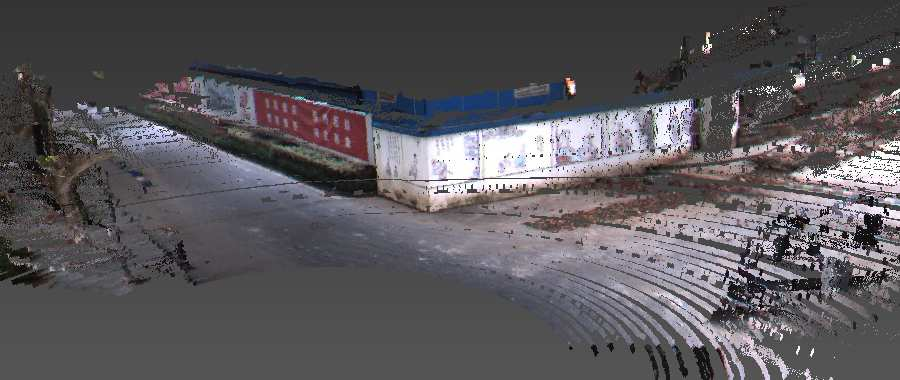
\includegraphics[width=\textwidth]{img/sensor_fusion/colored_point_cloud.png}
		\caption{Colored Point Cloud. Pixels are projected to the point cloud and nearby 3D points are colored with the colored of the correspondent pixel. Since \ac{lidar} \ac{fov} is bigger than camera, several points are black because no correspondences can be made. Source~\cite{Gong2013}}
		\label{fig:colored_point_cloud_example}
	\end{subfigure}
	\quad
	\begin{subfigure}[c]{0.40\textwidth}
		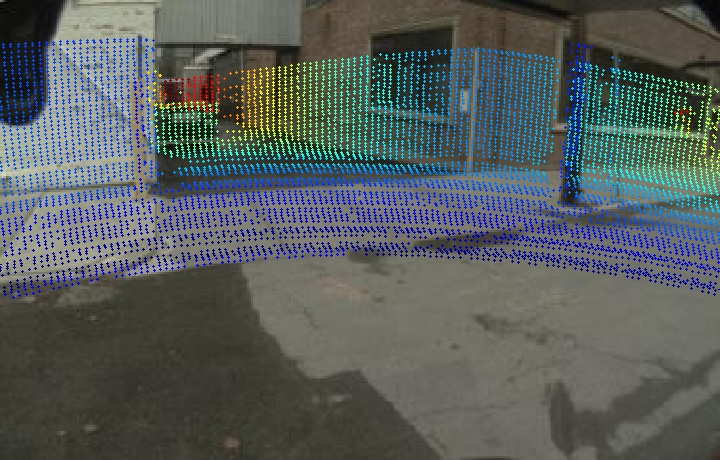
\includegraphics[width=\textwidth]{img/sensor_fusion/image_with_distance_point_cutted.png}
		\caption{Image with overlapping distance measurements. Point cloud points in the image \ac{fov} are projected into the image and colormap with intensity. Source~\cite{Bileschi2009}}
		\label{fig:image_with_lidar_distance}
	\end{subfigure}
	\caption{Examples of sensor fusion between camera and \ac{lidar} and the projection of camera color into the \ac{lidar} reference frame, augmenting its value (\subref{fig:colored_point_cloud_example}) and projecting distance information on camera image (\subref{fig:image_with_lidar_distance}).}
	\label{fig:point_cloud_camera_fusion_example}
\end{figure}

There are two major types of sensor fusion: 

\begin{enumerate}
	\item \textbf{Calibration + Fusion:} Sensors are first calibrated among themselves, using one of the techniques described on section~\ref{sec:sota:extrinsic_calibration}, and then data is converted to a referential of choice and merged;
	\item \textbf{Simultaneous Calibration and Fusion:} the implemented algorithms attempt to merge the data by minimizing some arbitrary cost function. The final result consists on the multimodal merged data and the extrinsic calibration parameters can be calculated;
	\item \textbf{``Direct'' Sensor Fusion:} Genetic algorithms, \ac{nn} or other similar tools analyze \ac{lidar} and camera data, without knowing any previous information about them, and outputs the merged data in the desired format.
\end{enumerate} 


\subsection{Calibration + Fusion}
For the first case, authors cited on section \nameref{sec:sota:extrinsic_calibration} shows the results of sensory fusion applied to the results of their calibration algorithms, as a proof of calibration correctness. 

Their sensor fusion technique is based on the application of the transformation described in equation~\ref{eq:jointRotationTranslationTransform}, which transforms data from the \ac{lidar} reference frame to the camera, allowing for a $3D point \leftrightarrow pixel$ mapping, enabling either point cloud coloring or overlapping the distance measurements on the image, as previously shown in figure~\ref{fig:point_cloud_camera_fusion_example}.
	
\begin{equation}
	\label{eq:jointRotationTranslationTransform}
	\begin{bmatrix}
		X_{cam} \\
		Y_{cam} \\
		Z_{cam} 
	\end{bmatrix}
	= 
		\underbrace{
	\left[
			\begin{array}{ccc|c}
				r_{xx} & r_{yx} & r_{zx} & t_x \\
					r_{xy} & r_{yy} & r_{zy} & t_y \\
					r_{xz} & r_{yz} & r_{zz} & t_z 
				\end{array}
		\right]
		}_\text{\large\textbf{[R|t]}}
	\begin{bmatrix}
		X_{LiDAR} \\
		Y_{LiDAR} \\
		Z_{LiDAR} 
	\end{bmatrix}
\end{equation}


\subsection{Simultaneous Calibration and Fusion}
Castorena \etal approach for sensor fusion matches the edges using a weighted total variation norm, that is also capable of providing additional information, useful not only for calibration, but also to refine the results of the fusion process and generate a more accurate colored point cloud~\cite{Castorena2016}.

Park \etal also proposes a method for fusion uncalibrated \ac{lidar} and stereo camera data, using two \ac{cnn}: one for calibration, by reducing error between disparity images; and a second to refine the fused disparity maps with the left image \cite{Park2019}. 

Li \etal proposes a method for simple indoor setups consisting of a single camera and a \ac{lidar} on a servo motor. The mechanism is rotated for three angular positions and a point cloud and image is taken for each one. Then, every image and point cloud are stitching together using fiducial features, resulting on a colored point cloud and on the determination of the calibration parameters~\cite{Li2016}. 

Yang \etal also proposes a method for stereo image and \ac{lidar} point cloud fusion using a Generalized \acl{icp} algorithm to match features and extracted a fused tridimensional refined model, at the same time it estimates the rigid body transform between camera and \ac{lidar}~\cite{Yang2017}.


\subsection{``Direct'' Sensor Fusion}
Liang \etal approach uses a multi-task multi-sensor dense fusion network for camera and \ac{lidar} fusion for object detection and 3D bounding box estimation.

Wei \etal for a real-time multi-sensor collision avoidance system develops a sensor fusion algorithm between a monocular camera and \ac{lidar} that uses \ac{cnn} and feature extraction to fuse \ac{lidar} and camera data for increasing the amount of beacons detected on a particular application~\cite{Wei2018}.


\section{Object Detection}
Object Detection is a field of \acl{cv} that intends to detect objects in image. Currently, two approaches to tackle this problem are possible:

\begin{enumerate}
	\item \textbf{\acl{ml} based approach:} objection detection is performed on two steps: first a set of feature descriptors are chosen and extracted from reference images; secondly a \acl{nn} takes those features and perform the classification;
	\item \textbf{Deep-Learning based approach:} end-to-end object detection without the need of specifying features.
\end{enumerate}

When referring to the first solution, Haar-like features~\cite{Messom2006}, \ac{sift}~\cite{Hughes2011a}, \ac{surf}~\cite{Bay2008} and \ac{hog}~\cite{Dalal2010, Surasak2018} features are normally used, on a Viola-Jones \ac{nn} (or its extensions)~\cite{Viola2001, ViolaP2004}. % For more details see 

The second solution is normally implemented with a Region Proposal \acf{cnn}, developed by Girshick on 2014 \etal~\cite{Girshick2014}. A common \ac{cnn} cannot be used on object detection on an image because the number of detected objects is variable, therefore the size of the output layer would also need to be, which is not possible on this architecture. A \ac{rcnn} differs from a \ac{cnn} due to the region proposal algorithm that precedes it, that limits the number of regions to be evaluated on an image to approximately 2000, therefore limiting the number of objects on an image~\cite{Girshick2014}. However, this \acl{nn} needs to be run for every one of the 2 thousand regions, making it slow and infeasible for real-time object detection~\cite{Girshick2014}. One year later, Girshick proposes a new architecture called Fast \ac{rcnn}, that runs the convolutional model only once and generates a feature map and bounding box offsets, increasing the speed of its \ac{rcnn} up to 20 times and improving \ac{map}~\cite{Girshick2015}. 

On 2016, Shaoqing Ren \etal proposes a newer architecture that does not use a selective search for the region proposal algorithm, but instead has a Region Proposal Network to generate \ac{roi} for the proposal classification stage, called Faster \ac{rcnn}~\cite{Ren2017}. Such architecture achieves state-of-the-art object detection at a frame-rate of 5 \ac{fps}. Alternative networks, such as \ac{spp} Deep \acl{cnn}~\cite{He2015}, will not be discussed here.

While the previous \ac{nn} use separated networks for region proposal of a possible object on an image and region classification to locate a possible object on an image, \ac{yolo}, developed by Joseph Redmon, is an alternative solution that analyzes the image only once, therefore keeping global context of the image while dividing it into regions and predicting bounding boxes. Those bounding boxes are weighted by the computed probabilities of each region and thresholding by the user~\cite{Redmon2016}. \ac{yolo}v2, released in 2017, at best can achieve, at best, 78.6 \ac{map} on the PASCAl VOC 2007 dataset at 40 \ac{fps} (see more details~\cite{Redmon2017}). \ac{yolo}v3, released in 2018, achieves at best, 57.9 \ac{map}-50 on COCOs dataset, at almost 20 \ac{fps} (3x faster than other networks with the same \ac{map}-50)~\cite{Redmon2018}.

\ac{yolo} runs on Darknet, an open source neural network framework written in C and \ac{cuda} of the same author~\cite{Redmon2013}.


\subsection{Platforms}
Several paid and cloud based alternatives exist, such as Amazon Rekognition~\cite{awsRekognition}, Google Could Vision \ac{api}~\cite{googlevision}, IBM Watson Visual Recognition~\cite{watson} and Microsoft Computer Vision software~\cite{azurecv}. 

Since those platforms are paid and required connection to the Internet, they are not good candidates to the solution we are trying to develop. Therefore, they are discarded.


\section{\ac{lidar} Interference}
\ac{tof} \ac{lidar}s basic principle implies that when a \ac{laser} pulse is emitted, three different scenarios are possible, being the first one the only one that produces a valid measurement:

\begin{enumerate}
\item The \ac{laser} pulse returns, due to the reflection of an obstacle;
\item The \ac{laser} pulse does not return;
\item The \ac{laser} pulse returns with intensity below the noise floor.
\end{enumerate}

Interference and crosstalk between the pairs of \acp{laser} and photodetectors on a \ac{lidar} are mitigated with different firing offsets, or in the case of mutual interference between \ac{lidar}, it is possible to synchronize their firing time using specialized clock signals \cite{vlp16}.

However, in a society when self-driving vehicles coexist, another scenario is possible: a \ac{lidar} `A'' fires a \ac{laser} pulse that is received, directly or indirectly, by the photodetector on a \ac{lidar} `B''. Since \ac{lidar} `B'' measures the distance to an obstacle by measuring the time between the firing and reception of its own \ac{laser} pulse, the reception of another \ac{laser} pulse results in an erroneous measure with an unpredictable behavior. If this interference is significant, the reliability of the \ac{lidar}, and consequently autonomous vehicles and \ac{adas}, is seriously undermined due to the incapability to accurately mapping their surroundings.

% This problem, deeply researched for automotive \ac{radar} \cite{}, as yet to gain the attention of the research community of automotive \ac{lidar} and 


To the best of the author knowledge, the first consideration about \ac{lidar} interference is given by Hebert and Krotkov in 1991~\cite{Hebert}. Their study was conducted for \ac{amcw} \ac{lidar} systems, and among other findings, they state that range and intensity measurements on \ac{lidar} are not completely independent, since lower intensity reflection can lead to an increase on range noise and shifts. 

Gunzung Kim \etal, in 2015, presents the first results on multiple \ac{lidar} interference on its three papers \cite{Kim2015a, Kim2015b, Kim2015c}. The three papers are based on a SICK LMS-511, a 2D \ac{lidar}\footnote{A single laser and photoreceptor are mounted on a rotating device, measuring several azimuthal angles when the motor rotates, but the polar angle is keep fixed, scanning a single line of the environment.}. Kim \etal setups consists on box with $5.3m \times 4m$ \cite{Kim2015a} or $5.3m \times 5.3m$ \cite{Kim2015b, Kim2015c}, where the \acp{lidar} are positioned. The walls are made of a low glossy wood. His classification of interference is based on the determination of a majorant and minorant for the distance of the wall, with a 10\% tolerance around the mean value.

% Kim \etal research despite using a 2D \ac{lidar} instead of a 3D \ac{lidar} is the only study to use two independent 2D \ac{lidar}s interfering with each other. Kim \etal results indicate that interference has spatial and temporal locality \cite{Kim2015} and in any given time, in Kim's setup, a data point has 0.05 \% probability of being interfered \cite{Kim2015}. The former states that if a particular angle is interfered, the following angles are likely to also be interfered; while the latter indicates that if a measure is interfered, on the following frame that same measure is also likely to be interfered. 

Kim \etal tests show the temporal and spatial locality of the data. Temporal locality implies that a given angular direction is more likely to be interfered if it was interfered in the past, indicating that interference persists through time. Spatial locality implies that for a current scan, if an interference occurs, it is more likely that the next angle will also be interfered, indicating that interference persists through space. 



The experiment conduct in~\cite{Kim2015a} captured a ground-truth model for 4 hours and the interference data on 50 hours. For a given angle, Kim research concluded that for his experimental setup, 4.4\% of the total number of full line scans were interfered, but that number only translate to one in each 2000 point (0.05\% interfered points for the total number o point registered). When considering the nature of interference, spatial interference is rare: 78\% of the interfered points are not interfered on their next measurement (against 15\% that are), and only 7\% of the angles are interfered consecutively 3 or more times, for a record of 13 (meaning 0.5seconds of interference). For consecutive interference on nearby azimuthal angles on the same scan, only 30\% of the interference happens a single angle and 26\% on a second. The largest consecutive number of angles with interference are 102, which translates to 25.5º.


On~\cite{Kim2015b}, Kim~\etal realized new tests on \ac{lidar} interference, adding two new tests: a side by side with a small displacement and a face to face test. On~\cite{Kim2015c} a back to back test is also performed. Note that despite the experimental setup \textit{Side by side \#1} being identical to the setup on~\cite{Kim2015a}, disagreements on all metrics occur. Therefore, for this test, the results discussed before~\cite{Kim2015a} and results presented on table~\ref{tab:kim_2015_results}, based on~\cite{Kim2015b, Kim2015c}, are not in agreement.

\begin{table}[H]
	\centering
	\renewcommand{\arraystretch}{1.3}
		\begin{tabular}{@{}l|c|c@{}}
			                 & \% of Lines Interfered & Relative Frequence of Interfered Points \\ \midrule
			Side by side \#1 & $1.795$                & $3.103\E^{-5}$  \\
			Side by side \#2 & $10.33$                & $1.667\E^{-4}$ \\
			Face to Face     & $1.433$                & $2.583\E^{-5}$  \\
			Back to Back A   & $0.211$                & $3.387\E^{-6}$  \\
			Back to Back B   & $0.216$                & $3.514\E^{-6}$  \\ \bottomrule
		\end{tabular}%
		\caption{Summary of Kim's \etal the interference results from \cite{Kim2015b, Kim2015c}, for all tests. On the second column, the percentage of lines with a single interfered point are presented and on the second column the relative frequency of interfered point for all the points measured}
	\label{tab:kim_2015_results}
\end{table}

The results of the second column, \textit{\% of Lines Interfered}, characterizes the number of lines on which interference as been found. For every test scenario on this column, the line interference caused are mostly non-consecutive (above 90\% for Face to Face and 94.3\% for all the other tests).

The third column, \textit{Relative Frequence of Interfered Points}, characterizes the number of measures that have been interfered regarding all measures made. Despite the maximum of consecutive spatial interference (4 scans), more than $99.7\%$ of all interferences happens isolated on a given azimuth, with no repetition on the next scan for the same interfered angle~\cite{Kim2015c}.



% To the best of the author's knowledge, despite the relevance of the topic to a society of self-driving cars, there are only three different studies available


In 2017, Kim \etal presents the results on the above papers \cite{Kim2015a, Kim2015b, Kim2015c}, extending its research by performing a intensity analysis~\cite{Kim2017}. His findings are that on a mutual interference scenario, the intensity of the received laser pulses varies significantly, confirming Hebert and Krotkov early findings that on a \ac{lidar} system range and intensity measures are not completely independent and interfering with one affects the results of other~\cite{Hebert}.

On the same paper, he also introduces a theoretical analysis of the multipath interference based on a Lambertian distribution for modelling the reflections on the walls~\cite{Kim2017}. The model lack generality, as it assumes average values for several parameters and some simplifications on the multipath interference, but allows to conclude that:

\begin{enumerate}
	\item After the second reflection on an obstacle, the attenuation suffered by the light ray is not sufficient for the receiving \ac{lidar} to detect it as an interference;
	\item Direct interference (on Kim's experimental setup and hardware) is likely to saturate the receptor of the interfered \ac{lidar}, which may or may not be considered a valid measurement by the hardware;
	\item Indirect interference with only one reflection can be interpreted as a valid measurement, since the intensity of the received interfered ray is similar to the intensity of valid measurement ray.
\end{enumerate}

On 2013, Retterath and Laumeyer \cite{Retterath2015}, seeking to provide an apparatus for an array based system with reduced interference. Their patented work is an array \ac{lidar} that was lower probability of crosstalk than other solutions, which was latter patented worldwide~\cite{Retterath2015WO}. On 2016, another patent is filled for the same array based \ac{lidar}~\cite{Retterath2016}, this time for object detection and in 2017, Facet Technology, the patent applicant, sends out a Press Release indicating that they have been developed a \textit{``Safe and Secure\acs{lidar}\textregistered Crosstalk Elimination Licensing Program''}, and that they have experienced crosstalk interferences up 2\%~\cite{Facet}.

Jonathan Petit \etal present a study on how to remote attack automotive cameras and \acp{lidar} on vehicles~\cite{Petit2015}. For \ac{lidar} relay, replaying and spoofing attacks are explained. Petit's work shows, for laboratory scenarios, how to make obstacles disappear and how to make the \ac{lidar} see ``ghost'' objects, for distances further than the distance of the spoofer. Hocheol Shin \etal, two years later, presents an improved method that not only is able to spoof obstacles at a distance further than the distance of the spoofer, but also closer~\cite{Shin2017}. His work used more commonly used \acp{lidar}, such as Velodyne VLP-16~\cite{vlp16}. Shin \etal also find that the curved reception glass of \acp{lidar} allow for reflection of an attacking light source inside its case, allowing the attacker to be at a different direction that of the perceived attack. Despite their work being extremely experimental, and laser alignment required for an effective attack on real driving scenarios, Petit \etal and Shin \etal research show that such result is possible. Some results from Shin research are shown on figure~\ref{fig:shinInterference}.

\begin{figure}[H]
	\centering
	\begin{subfigure}[c]{0.4\textwidth}
	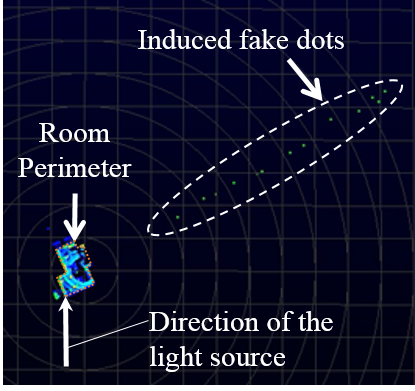
\includegraphics[width=\textwidth]{img/lidar/interference_angle_control.png}
		\caption{Spoofing an obstacle at a different angle of the spoofer}
		\label{fig:shinInterferenceAngle}
	\end{subfigure}
	\quad
	\begin{subfigure}[c]{0.55\textwidth}
		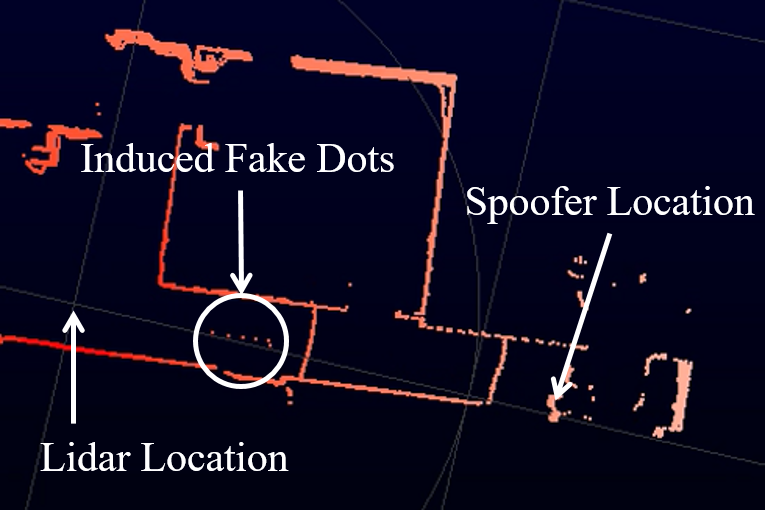
\includegraphics[width=\textwidth]{img/lidar/interference_distance_control.png}
		\caption{Spoofing an obstacle at a closer distance than the spoofer}
		\label{fig:shinInterferenceDistance}
	\end{subfigure}
	\caption{Spoofing examples on a Velodyne VLP-16 \ac{lidar}. Source~\cite{Shin2017}}
	\label{fig:shinInterference}
\end{figure}


On 2017, Velodyne Inc., one of the major manufacturer of \ac{lidar}, filled a patent on a new implementation that reduced crosstalk~\cite{Hall2017}. Their focus was to solve multi-channel crosstalk, but multi-\ac{lidar} crosstalk reduction is also referred on the patent.

Axel Diehm \etal, on 2018, proposes a spatial temporal filter for eliminating a crosstalk problem between two Velodyne HDL-64 \acp{lidar}~\cite{Hebel2018}. Their crosstalk behaviour is well defined as a area of interfered points at a particular orientation, and their work is focused on how to filter out those points and partially expanded their analysis to the time domain of interference, instead of searching to understand the behaviour that is causing them.

On 2019, Gerald Popko \etal presents a mathematical description on how stationary, coplanar and circular 2D scanning \ac{lidar} can interfere through beam path interference of the optical \ac{fov}, see~\cite{Popko2019a}. Based on his description, he repeats Kim's \etal experiments proposing a new statistical interference detector, instead of Kim's maximum distance minorant and majorant~\cite{Kim2015a}, and also performs a Monte-Carlo simulation~\cite{Popko2019b}. Popko \etal findings are that:

\begin{enumerate}
	\item The interference behavior depends majorly on the target geometry and beam intersection, and not on radiometric considerations;
	\item Simulating the \ac{lidar} interference can only provide good qualitative results, since only the scattered interference provided a value closed to the real value measured;
	\item The direct interference is dominant over the scattering interference;
	\item The direct interference is mainly responsible for small distance measurement errors, while scattering interference is mainly present for large distance measurement errors;
\end{enumerate}

Lastly, Popko \etal interference results are two orders of magnitude higher than Kim's \etal measurements, $1.041 \%$~\cite{Popko2019b} vs $0.05\%$~\cite{Kim2015a}.

